\chapter{Implementation}

\section{Architecture}

\begin{figure}[h]
\centering
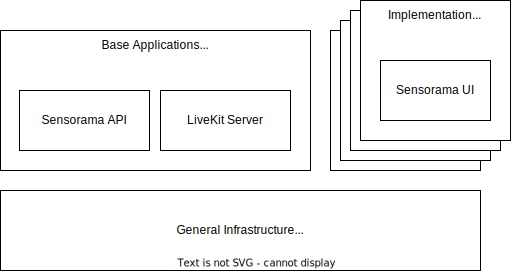
\includegraphics[scale=0.5]{04_Artefakte/01_Abbildungen/sensorama-stack}
\caption[{Sensorama Stack Diagram}]{The main components comprising the application architecture\protect}
\label{fig:sensoramaStack}
\end{figure}

\subsection{Hardware}

\subsection{Software}


\section{Application infrastructure}

While all the frameworks represented in \ref{fig:mostUsedFrameworks} could be used to build an application as envisioned in this study, Vue is selected as the tool of choice, both due to the relatively high acceptance and the comparably steep learning curve. Additionally, it is already used in a number of applications designed by the author.

\subsection{WebRTC Server}

\subsection{Database}

\section{Design Paradigms}

\subsection{Application Partitioning}

\subsection{Coding Style}

\subsection{Testing}

\section{Application Components}

\subsection{Web Frontend}

\subsection{API Backend}

\subsection{Native Utilities}
